% Options for packages loaded elsewhere
\PassOptionsToPackage{unicode}{hyperref}
\PassOptionsToPackage{hyphens}{url}
%
\documentclass[
]{article}
\usepackage{amsmath,amssymb}
\usepackage{iftex}
\ifPDFTeX
  \usepackage[T1]{fontenc}
  \usepackage[utf8]{inputenc}
  \usepackage{textcomp} % provide euro and other symbols
\else % if luatex or xetex
  \usepackage{unicode-math} % this also loads fontspec
  \defaultfontfeatures{Scale=MatchLowercase}
  \defaultfontfeatures[\rmfamily]{Ligatures=TeX,Scale=1}
\fi
\usepackage{lmodern}
\ifPDFTeX\else
  % xetex/luatex font selection
\fi
% Use upquote if available, for straight quotes in verbatim environments
\IfFileExists{upquote.sty}{\usepackage{upquote}}{}
\IfFileExists{microtype.sty}{% use microtype if available
  \usepackage[]{microtype}
  \UseMicrotypeSet[protrusion]{basicmath} % disable protrusion for tt fonts
}{}
\makeatletter
\@ifundefined{KOMAClassName}{% if non-KOMA class
  \IfFileExists{parskip.sty}{%
    \usepackage{parskip}
  }{% else
    \setlength{\parindent}{0pt}
    \setlength{\parskip}{6pt plus 2pt minus 1pt}}
}{% if KOMA class
  \KOMAoptions{parskip=half}}
\makeatother
\usepackage{xcolor}
\usepackage[margin=1in]{geometry}
\usepackage{color}
\usepackage{fancyvrb}
\newcommand{\VerbBar}{|}
\newcommand{\VERB}{\Verb[commandchars=\\\{\}]}
\DefineVerbatimEnvironment{Highlighting}{Verbatim}{commandchars=\\\{\}}
% Add ',fontsize=\small' for more characters per line
\usepackage{framed}
\definecolor{shadecolor}{RGB}{248,248,248}
\newenvironment{Shaded}{\begin{snugshade}}{\end{snugshade}}
\newcommand{\AlertTok}[1]{\textcolor[rgb]{0.94,0.16,0.16}{#1}}
\newcommand{\AnnotationTok}[1]{\textcolor[rgb]{0.56,0.35,0.01}{\textbf{\textit{#1}}}}
\newcommand{\AttributeTok}[1]{\textcolor[rgb]{0.13,0.29,0.53}{#1}}
\newcommand{\BaseNTok}[1]{\textcolor[rgb]{0.00,0.00,0.81}{#1}}
\newcommand{\BuiltInTok}[1]{#1}
\newcommand{\CharTok}[1]{\textcolor[rgb]{0.31,0.60,0.02}{#1}}
\newcommand{\CommentTok}[1]{\textcolor[rgb]{0.56,0.35,0.01}{\textit{#1}}}
\newcommand{\CommentVarTok}[1]{\textcolor[rgb]{0.56,0.35,0.01}{\textbf{\textit{#1}}}}
\newcommand{\ConstantTok}[1]{\textcolor[rgb]{0.56,0.35,0.01}{#1}}
\newcommand{\ControlFlowTok}[1]{\textcolor[rgb]{0.13,0.29,0.53}{\textbf{#1}}}
\newcommand{\DataTypeTok}[1]{\textcolor[rgb]{0.13,0.29,0.53}{#1}}
\newcommand{\DecValTok}[1]{\textcolor[rgb]{0.00,0.00,0.81}{#1}}
\newcommand{\DocumentationTok}[1]{\textcolor[rgb]{0.56,0.35,0.01}{\textbf{\textit{#1}}}}
\newcommand{\ErrorTok}[1]{\textcolor[rgb]{0.64,0.00,0.00}{\textbf{#1}}}
\newcommand{\ExtensionTok}[1]{#1}
\newcommand{\FloatTok}[1]{\textcolor[rgb]{0.00,0.00,0.81}{#1}}
\newcommand{\FunctionTok}[1]{\textcolor[rgb]{0.13,0.29,0.53}{\textbf{#1}}}
\newcommand{\ImportTok}[1]{#1}
\newcommand{\InformationTok}[1]{\textcolor[rgb]{0.56,0.35,0.01}{\textbf{\textit{#1}}}}
\newcommand{\KeywordTok}[1]{\textcolor[rgb]{0.13,0.29,0.53}{\textbf{#1}}}
\newcommand{\NormalTok}[1]{#1}
\newcommand{\OperatorTok}[1]{\textcolor[rgb]{0.81,0.36,0.00}{\textbf{#1}}}
\newcommand{\OtherTok}[1]{\textcolor[rgb]{0.56,0.35,0.01}{#1}}
\newcommand{\PreprocessorTok}[1]{\textcolor[rgb]{0.56,0.35,0.01}{\textit{#1}}}
\newcommand{\RegionMarkerTok}[1]{#1}
\newcommand{\SpecialCharTok}[1]{\textcolor[rgb]{0.81,0.36,0.00}{\textbf{#1}}}
\newcommand{\SpecialStringTok}[1]{\textcolor[rgb]{0.31,0.60,0.02}{#1}}
\newcommand{\StringTok}[1]{\textcolor[rgb]{0.31,0.60,0.02}{#1}}
\newcommand{\VariableTok}[1]{\textcolor[rgb]{0.00,0.00,0.00}{#1}}
\newcommand{\VerbatimStringTok}[1]{\textcolor[rgb]{0.31,0.60,0.02}{#1}}
\newcommand{\WarningTok}[1]{\textcolor[rgb]{0.56,0.35,0.01}{\textbf{\textit{#1}}}}
\usepackage{graphicx}
\makeatletter
\def\maxwidth{\ifdim\Gin@nat@width>\linewidth\linewidth\else\Gin@nat@width\fi}
\def\maxheight{\ifdim\Gin@nat@height>\textheight\textheight\else\Gin@nat@height\fi}
\makeatother
% Scale images if necessary, so that they will not overflow the page
% margins by default, and it is still possible to overwrite the defaults
% using explicit options in \includegraphics[width, height, ...]{}
\setkeys{Gin}{width=\maxwidth,height=\maxheight,keepaspectratio}
% Set default figure placement to htbp
\makeatletter
\def\fps@figure{htbp}
\makeatother
\setlength{\emergencystretch}{3em} % prevent overfull lines
\providecommand{\tightlist}{%
  \setlength{\itemsep}{0pt}\setlength{\parskip}{0pt}}
\setcounter{secnumdepth}{-\maxdimen} % remove section numbering
\ifLuaTeX
  \usepackage{selnolig}  % disable illegal ligatures
\fi
\IfFileExists{bookmark.sty}{\usepackage{bookmark}}{\usepackage{hyperref}}
\IfFileExists{xurl.sty}{\usepackage{xurl}}{} % add URL line breaks if available
\urlstyle{same}
\hypersetup{
  pdftitle={Lab 1},
  pdfauthor={Irimie Fabio},
  hidelinks,
  pdfcreator={LaTeX via pandoc}}

\title{Lab 1}
\usepackage{etoolbox}
\makeatletter
\providecommand{\subtitle}[1]{% add subtitle to \maketitle
  \apptocmd{\@title}{\par {\large #1 \par}}{}{}
}
\makeatother
\subtitle{Exercise 2}
\author{Irimie Fabio}
\date{}

\begin{document}
\maketitle

{
\setcounter{tocdepth}{2}
\tableofcontents
}
\hypertarget{a}{%
\subsection{A}\label{a}}

Create 2 vectos twice: using the colon oprator and the seq(function)

vec1: 1, 2, 3, 4, 5, 6, 7, 8, 9, 10

vec2: 2, 7, 12

\begin{Shaded}
\begin{Highlighting}[]
\NormalTok{vec1 }\OtherTok{\textless{}{-}} \DecValTok{1}\SpecialCharTok{:}\DecValTok{10}
\FunctionTok{cat}\NormalTok{(}\StringTok{"Vec1.1: "}\NormalTok{, vec1, }\StringTok{"}\SpecialCharTok{\textbackslash{}n}\StringTok{"}\NormalTok{)}
\DocumentationTok{\#\# Vec1.1:  1 2 3 4 5 6 7 8 9 10}
\NormalTok{vec1 }\OtherTok{\textless{}{-}} \FunctionTok{seq}\NormalTok{(}\DecValTok{1}\NormalTok{, }\DecValTok{10}\NormalTok{, }\DecValTok{1}\NormalTok{)}
\FunctionTok{cat}\NormalTok{(}\StringTok{"Vec1.2: "}\NormalTok{, vec1, }\StringTok{"}\SpecialCharTok{\textbackslash{}n}\StringTok{"}\NormalTok{)}
\DocumentationTok{\#\# Vec1.2:  1 2 3 4 5 6 7 8 9 10}

\NormalTok{vec2 }\OtherTok{\textless{}{-}}\NormalTok{ (}\DecValTok{1}\SpecialCharTok{:}\DecValTok{12}\NormalTok{)[}\SpecialCharTok{{-}}\FunctionTok{c}\NormalTok{(}\DecValTok{1}\NormalTok{, }\DecValTok{3}\SpecialCharTok{:}\DecValTok{6}\NormalTok{, }\DecValTok{8}\SpecialCharTok{:}\DecValTok{11}\NormalTok{)]}
\FunctionTok{cat}\NormalTok{(}\StringTok{"Vec2.1: "}\NormalTok{, vec2, }\StringTok{"}\SpecialCharTok{\textbackslash{}n}\StringTok{"}\NormalTok{)}
\DocumentationTok{\#\# Vec2.1:  2 7 12}
\NormalTok{vec2 }\OtherTok{\textless{}{-}} \FunctionTok{seq}\NormalTok{(}\DecValTok{2}\NormalTok{, }\DecValTok{12}\NormalTok{, }\DecValTok{5}\NormalTok{)}
\FunctionTok{cat}\NormalTok{(}\StringTok{"Vec2.2: "}\NormalTok{, vec2, }\StringTok{"}\SpecialCharTok{\textbackslash{}n}\StringTok{"}\NormalTok{)}
\DocumentationTok{\#\# Vec2.2:  2 7 12}
\end{Highlighting}
\end{Shaded}

\hypertarget{b}{%
\subsection{B}\label{b}}

Create a 4x2 matrix of all zeros and store it in a variable (mymat).
Then, replace the second row in the matrix with a vector consisting of a
3 and a 6.

\begin{Shaded}
\begin{Highlighting}[]
\NormalTok{mymat }\OtherTok{\textless{}{-}} \FunctionTok{matrix}\NormalTok{(}
  \DecValTok{0}\NormalTok{,}
  \DecValTok{4}\NormalTok{,}
  \DecValTok{2}
\NormalTok{)}
\FunctionTok{cat}\NormalTok{(}\StringTok{"Starting matrix:}\SpecialCharTok{\textbackslash{}n}\StringTok{"}\NormalTok{)}
\DocumentationTok{\#\# Starting matrix:}
\NormalTok{mymat}
\DocumentationTok{\#\#      [,1] [,2]}
\DocumentationTok{\#\# [1,]    0    0}
\DocumentationTok{\#\# [2,]    0    0}
\DocumentationTok{\#\# [3,]    0    0}
\DocumentationTok{\#\# [4,]    0    0}
\NormalTok{mymat[}\DecValTok{2}\NormalTok{, }\DecValTok{1}\NormalTok{] }\OtherTok{\textless{}{-}} \DecValTok{3}
\NormalTok{mymat[}\DecValTok{2}\NormalTok{, }\DecValTok{2}\NormalTok{] }\OtherTok{\textless{}{-}} \DecValTok{6}
\FunctionTok{cat}\NormalTok{(}\StringTok{"Replaced matrix:}\SpecialCharTok{\textbackslash{}n}\StringTok{"}\NormalTok{)}
\DocumentationTok{\#\# Replaced matrix:}
\NormalTok{mymat}
\DocumentationTok{\#\#      [,1] [,2]}
\DocumentationTok{\#\# [1,]    0    0}
\DocumentationTok{\#\# [2,]    3    6}
\DocumentationTok{\#\# [3,]    0    0}
\DocumentationTok{\#\# [4,]    0    0}
\end{Highlighting}
\end{Shaded}

\hypertarget{c}{%
\subsection{C}\label{c}}

Create a vector x which consists of 20 equally spaced points in the
range from \(-\pi\) to \(+\pi\). Create a y vector which is sin(x).

\begin{Shaded}
\begin{Highlighting}[]
\NormalTok{x }\OtherTok{\textless{}{-}} \FunctionTok{seq}\NormalTok{(}\SpecialCharTok{{-}}\NormalTok{pi, pi, }\AttributeTok{length.out =} \DecValTok{20}\NormalTok{)}
\NormalTok{x}
\DocumentationTok{\#\#  [1] {-}3.1415927 {-}2.8108987 {-}2.4802047 {-}2.1495108 {-}1.8188168 {-}1.4881228}
\DocumentationTok{\#\#  [7] {-}1.1574289 {-}0.8267349 {-}0.4960409 {-}0.1653470  0.1653470  0.4960409}
\DocumentationTok{\#\# [13]  0.8267349  1.1574289  1.4881228  1.8188168  2.1495108  2.4802047}
\DocumentationTok{\#\# [19]  2.8108987  3.1415927}

\NormalTok{y }\OtherTok{\textless{}{-}} \FunctionTok{sin}\NormalTok{(x)}
\NormalTok{y}
\DocumentationTok{\#\#  [1] {-}1.224647e{-}16 {-}3.246995e{-}01 {-}6.142127e{-}01 {-}8.371665e{-}01}
\DocumentationTok{\#\#  [5] {-}9.694003e{-}01 {-}9.965845e{-}01 {-}9.157733e{-}01 {-}7.357239e{-}01}
\DocumentationTok{\#\#  [9] {-}4.759474e{-}01 {-}1.645946e{-}01  1.645946e{-}01  4.759474e{-}01}
\DocumentationTok{\#\# [13]  7.357239e{-}01  9.157733e{-}01  9.965845e{-}01  9.694003e{-}01}
\DocumentationTok{\#\# [17]  8.371665e{-}01  6.142127e{-}01  3.246995e{-}01  1.224647e{-}16}
\end{Highlighting}
\end{Shaded}

\hypertarget{d}{%
\subsection{D}\label{d}}

Create a 4x6 matrix of random integers, each in the range from -5 to 5;
store it in a variable (mat). Create another matrix that stores for each
element the absolute value of the corresponding element in the original
matrix (mat\_pos).

\begin{Shaded}
\begin{Highlighting}[]
\NormalTok{mat }\OtherTok{\textless{}{-}} \FunctionTok{matrix}\NormalTok{(}
  \FunctionTok{round}\NormalTok{(}\FunctionTok{runif}\NormalTok{(}\DecValTok{4} \SpecialCharTok{*} \DecValTok{6}\NormalTok{, }\SpecialCharTok{{-}}\DecValTok{5}\NormalTok{, }\DecValTok{5}\NormalTok{), }\AttributeTok{digits =} \DecValTok{0}\NormalTok{),}
  \DecValTok{4}\NormalTok{,}
  \DecValTok{6}
\NormalTok{)}
\NormalTok{mat\_pos }\OtherTok{\textless{}{-}} \FunctionTok{abs}\NormalTok{(mat)}

\NormalTok{mat}
\DocumentationTok{\#\#      [,1] [,2] [,3] [,4] [,5] [,6]}
\DocumentationTok{\#\# [1,]    3    5   {-}4    3    2    2}
\DocumentationTok{\#\# [2,]   {-}3   {-}2   {-}2   {-}3    1    3}
\DocumentationTok{\#\# [3,]    3    3   {-}2    3    3    3}
\DocumentationTok{\#\# [4,]   {-}4   {-}2    4    4    4    2}
\NormalTok{mat\_pos}
\DocumentationTok{\#\#      [,1] [,2] [,3] [,4] [,5] [,6]}
\DocumentationTok{\#\# [1,]    3    5    4    3    2    2}
\DocumentationTok{\#\# [2,]    3    2    2    3    1    3}
\DocumentationTok{\#\# [3,]    3    3    2    3    3    3}
\DocumentationTok{\#\# [4,]    4    2    4    4    4    2}
\end{Highlighting}
\end{Shaded}

\hypertarget{e}{%
\subsection{E}\label{e}}

Plot exp(x) for values of x ranging from -2 to 2 in steps of 0.1. Put an
appropriate title on the plot, and label the axes.

\begin{Shaded}
\begin{Highlighting}[]
\NormalTok{x }\OtherTok{\textless{}{-}} \FunctionTok{seq}\NormalTok{(}\SpecialCharTok{{-}}\DecValTok{2}\NormalTok{, }\DecValTok{2}\NormalTok{, }\FloatTok{0.1}\NormalTok{)}
\NormalTok{y }\OtherTok{\textless{}{-}} \FunctionTok{exp}\NormalTok{(x)}
\FunctionTok{plot}\NormalTok{(x, y,}
  \AttributeTok{type =} \StringTok{"l"}\NormalTok{,}
  \AttributeTok{xlab =} \StringTok{"x"}\NormalTok{,}
  \AttributeTok{ylab =} \StringTok{"y"}\NormalTok{,}
  \AttributeTok{main =} \StringTok{"Exponential function"}
\NormalTok{)}
\end{Highlighting}
\end{Shaded}

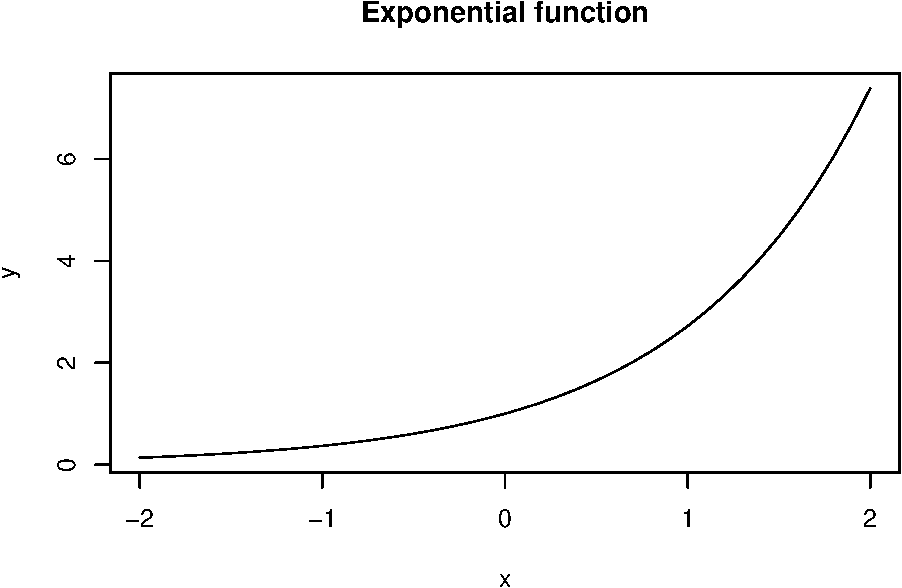
\includegraphics{es2_files/figure-latex/unnamed-chunk-5-1.pdf}

\hypertarget{f}{%
\subsection{F}\label{f}}

Create a vector x with values ranging from 1 to 100 in steps of 5.
Create a vector y which is the square root of each value in x. Plot
these points. Now, use the barplot() function instead of plot() to get a
bar chart. Keep both plots together.

\begin{Shaded}
\begin{Highlighting}[]
\NormalTok{x }\OtherTok{\textless{}{-}} \FunctionTok{seq}\NormalTok{(}\DecValTok{1}\NormalTok{, }\DecValTok{100}\NormalTok{, }\DecValTok{5}\NormalTok{)}
\NormalTok{y }\OtherTok{\textless{}{-}} \FunctionTok{sqrt}\NormalTok{(x)}
\FunctionTok{par}\NormalTok{(}\AttributeTok{mfrow =} \FunctionTok{c}\NormalTok{(}\DecValTok{1}\NormalTok{, }\DecValTok{2}\NormalTok{))}
\FunctionTok{plot}\NormalTok{(x, y)}
\FunctionTok{barplot}\NormalTok{(x, y)}
\end{Highlighting}
\end{Shaded}

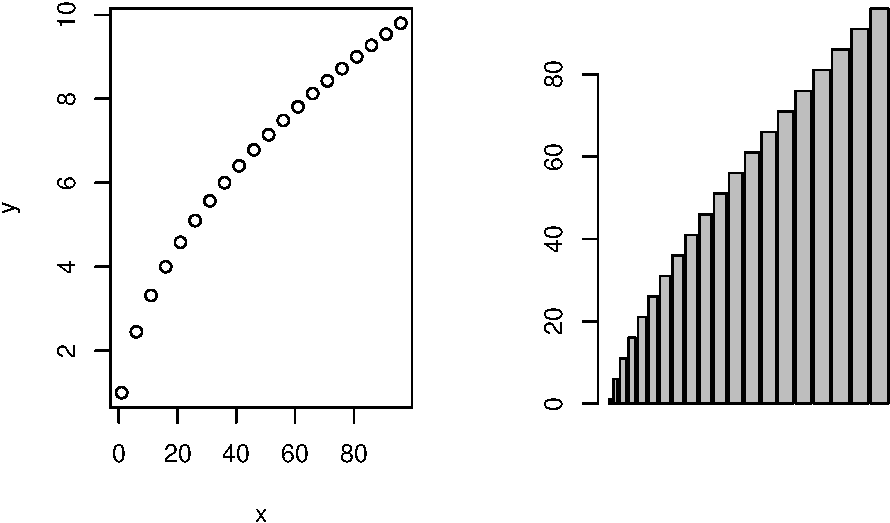
\includegraphics{es2_files/figure-latex/unnamed-chunk-6-1.pdf}

\end{document}
